 \documentclass{article}
\usepackage[utf8]{inputenc}
\usepackage{graphicx}
\usepackage[margin=1in]{geometry}
\usepackage[justification=centering]{caption}
\usepackage{setspace}
\bibliographystyle{chicago}
\usepackage{hyperref}
\usepackage{natbib}
\usepackage{indentfirst}
\usepackage{lscape}


\doublespacing
\title{The Psychology of State Repression: Replication}
\author{Haseeb Bajwa, John Mathews, Rithika Kumar}
\date{\today}

\begin{document}

\maketitle

\section*{Overview of Paper and Research Design}

We examine Lauren Young$'$s (\citeyear{young2019psychology}) paper titled ``The psychology of state repression: Fear and dissent decisions in Zimbabwe." She conducts an experiment to see how fear affects the level of dissent in people’s behavior. The logic of the experiment is to how understand how fear is used in dictatorship to both conform and dissent from behavior expected by the authoritarian regime. We obtained the dataset from Harvard dataverse and used that to generate the tables and figures in this paper.

Adopting an emotional induction experiment commonly used in psychology, \footnote{Often called an affective emotional memory task (AEMT)} respondents were asked to reflect upon and describe a situation that makes her relaxed (control) or afraid (treatment) in detail and in a way that would make another individual feel the emotion. Half of the treatment respondents were asked to describe fears around politics and elections, reflecting on the frightening things related to dissent decision and behavior. Conversely, the other half of treatment respondents were asked to describe general fears that are not related to experiences with politics and elections, such as snakes, witchcraft, and walking in the dark. Following the emotional induction, respondents were asked a series of 12 questions on their propensity to participate in dissent (hypothetical measure) and to choose between a plastic wristband with a pro-democracy slogan or another plain wristband as a gift for participating in the study (behavioral measure). The wristbands are similar in appearance and value, thus choosing the political wristband can be interpreted as participation in an act of dissent.

\clearpage


%%% SECTION 1

\section{Summary Statistics and Balance on Baseline Covariates}

%%% Table 1
\begin{table}[ht]
\label{summarybal}
\caption{Summary Statistics and Balance on Baseline Covariates}
\centering
\scalebox{1}{\begin{tabular}{rrrrrrrr}
  \hline
   & \multicolumn{3}{c}{\textit{Mean}} & \multicolumn{2}{c}{\textit{Difference}}& \multicolumn{2}{c}{\textit{p-value}}\\ 
\cline{2-4} \cline{5-6} \cline{7-8} 
\\[-4.8ex]  \\ 
 & C & T_{GF} & T_{PF} & T_{GF} - C & T_{PF} - C & T_{GF} - C & T_{PF} - C \\ 
  \hline
Female & 0.53 & 0.51 & 0.51 & 0.02 & 0.02 & 0.72 & 0.71 \\ 
  Education (4-pt scale) & 1.74 & 1.65 & 1.74 & 0.09 & -0.00 & 0.18 & 0.98 \\ 
  Age & 37.74 & 37.92 & 37.95 & -0.18 & -0.21 & 0.89 & 0.87 \\ 
  Assets: Generator & 0.20 & 0.18 & 0.21 & 0.02 & -0.01 & 0.63 & 0.76 \\ 
  Assets: Smartphone & 0.38 & 0.31 & 0.38 & 0.07 & -0.00 & 0.10 & 0.97 \\ 
  Assets: Electricity & 0.41 & 0.41 & 0.46 & 0.00 & -0.05 & 1.00 & 0.33 \\ 
  Assets: Bicycle & 0.22 & 0.23 & 0.21 & -0.01 & 0.01 & 0.83 & 0.78 \\ 
  Assets: Chickens & 0.51 & 0.54 & 0.45 & -0.03 & 0.06 & 0.55 & 0.20 \\ 
  Assets: Cattle & 0.33 & 0.31 & 0.28 & 0.02 & 0.05 & 0.60 & 0.24 \\ 
  Income (USD) per HH & 109.13 & 103.59 & 113.83 & 5.55 & -4.69 & 0.63 & 0.71 \\ 
   \hline
\end{tabular}}
\begin{tablenotes}
      \small
      \item C refers to the control group, T\textsubscript{GF} refers to the general fear treatment, and T\textsubscript{PF} refers to the political fear treatment.
    \end{tablenotes}
\end{table}

Table 1 presents the summary statistics and tests whether treatment assignment was balanced across multiple covariates such as gender, education level, age, asset ownership, and household income. The p-values suggest that there is no statistically significant difference between the control group and general fear treatment group, as well as between the control group and the political fear treatment group.

\subsection{Manipulation Checks}

Figure 1 shows the manipulation checks that test the extent to which the reflection tasks induced fear and five other primary emotions, namely anger, disgust, sadness, surprise, and happiness. In practice, multiple emotions are triggered upon the activation of one emotion, thus the authors wanted to make sure that the fear treatment causes positive change in similarly related emotions and has the opposite effect on happiness. This is evident from the bar graphs in Figure 1, where the treatment of general and political fear triggered emotions of anger, disgust, sadness, and surprise in addition to fear and at the same time finding a negative result for happiness. 
\clearpage

%% Figure 1

\begin{figure}[!htbp]
\label{emotions}
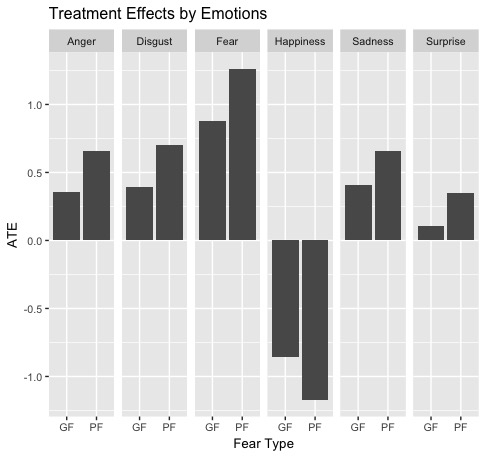
\includegraphics[scale=0.9]{Fig1.png}
\caption{The bar graphs show that fear treatments elicits positive change in related emotions and has the opposite effect on happiness. The differences in emotions are significant which shows that the treatment was able to successfully manipulate people's emotions.}
\centering
\end{figure}



%%% Section 2

\section{Fear Treatment Reduces Dissent}

%%% Table 2

\begin{table}[!htbp] \centering 
  \caption{Fear Treatment Reduces Dissent} 
  \label{ATEfeardissent} 
\scalebox{0.8}{\begin{tabular}{@{\extracolsep{5pt}}lcccc} 
\\[-1.8ex]\hline 
\hline \\[-1.8ex] 
 & \multicolumn{2}{c}{Hypothetical} & \multicolumn{2}{c}{Behavioral} \\ 
 \hline \\[-1.8ex]
\\[-1.8ex] & General Fear & Political Fear & General Fear & Political Fear\\ 
\\[-1.8ex] & (1) & (2) & (3) & (4)\\ 
\hline \\[-1.8ex] 
ATEs & -0.545 & -0.773 & -0.104 & -0.189 \\ 
SE & (0.077) & (0.080) & (0.050) & (0.053) \\
RI p-value & $<$ 0.001 & $<$ 0.001 & 0.03521 & 0.00016 \\ 
N & 484 & 486 & 329 & 326 \\ 
Sample & \multicolumn{2}{c}{All} & \multicolumn{2}{c}{Wristband} \\
\hline 
\hline \\[-1.8ex] 
\end{tabular}}
\begin{tablenotes}
      \small
\item Notes: The first row presents the estimated Average Treatment Effects (ATEs) of the general and political fear treatments in the hypothesis measure of propensity to dissent in Columns 1-2, and the behavioral measure in Columns 3-4. ATEs are calculated based on assignment to treatment and weighted by inverse propensity scores by block.
\end{tablenotes}
\end{table} 

The estimated average treatment effect (ATE) of the general and political fear treatments on the hypothetical and behavior measure of propensity to dissent is presented in Table \ref{ATEfeardissent}. It shows that respondents who receive the fear treatment are less likely to express dissent and are less likely to take the wristband with the pro-democracy slogan. The effects are statistically significant. 

The general and political fear treatments reduced the likelihood that respondents said they were to take action on the hypothetical dissent measure by 0.55 and 0.77 standard deviation respectively. On the other hand, the general and political fear treatments reduced the proportion of respondents who took the wristband by 10 and 19 percentage points respectively. The substantive interpretations for the hypothetical and behavioral measures are different because the former is based on an index of 12 questions while the latter is a binary outcome. 

%%% SECTION 3

\section{Substantive Differences in Dissent by Treatment Groups}

In addition to the main results, the author also shows substantive differences between participants in the control and fear condition when asked questions on daily actions involving six political activities. Figure 1 below shows that both "General fear (TG)" and "Political fear (TF)" cause a substantial decrease in dissenting behavior even in indirect political activities. For example, a 28\% of people in the control group said that they were very likely or sure to share a joke abut the president during an election period. However, this number drops to 7-8\% in the fear treatment groups. Similar results are found for the other political activities. This shows that fear induces changes in dissenting behavior beyond the political realm and has substantive effects on people living under such regimes. 

%%% Figure 2
\begin{figure}[!htbp]
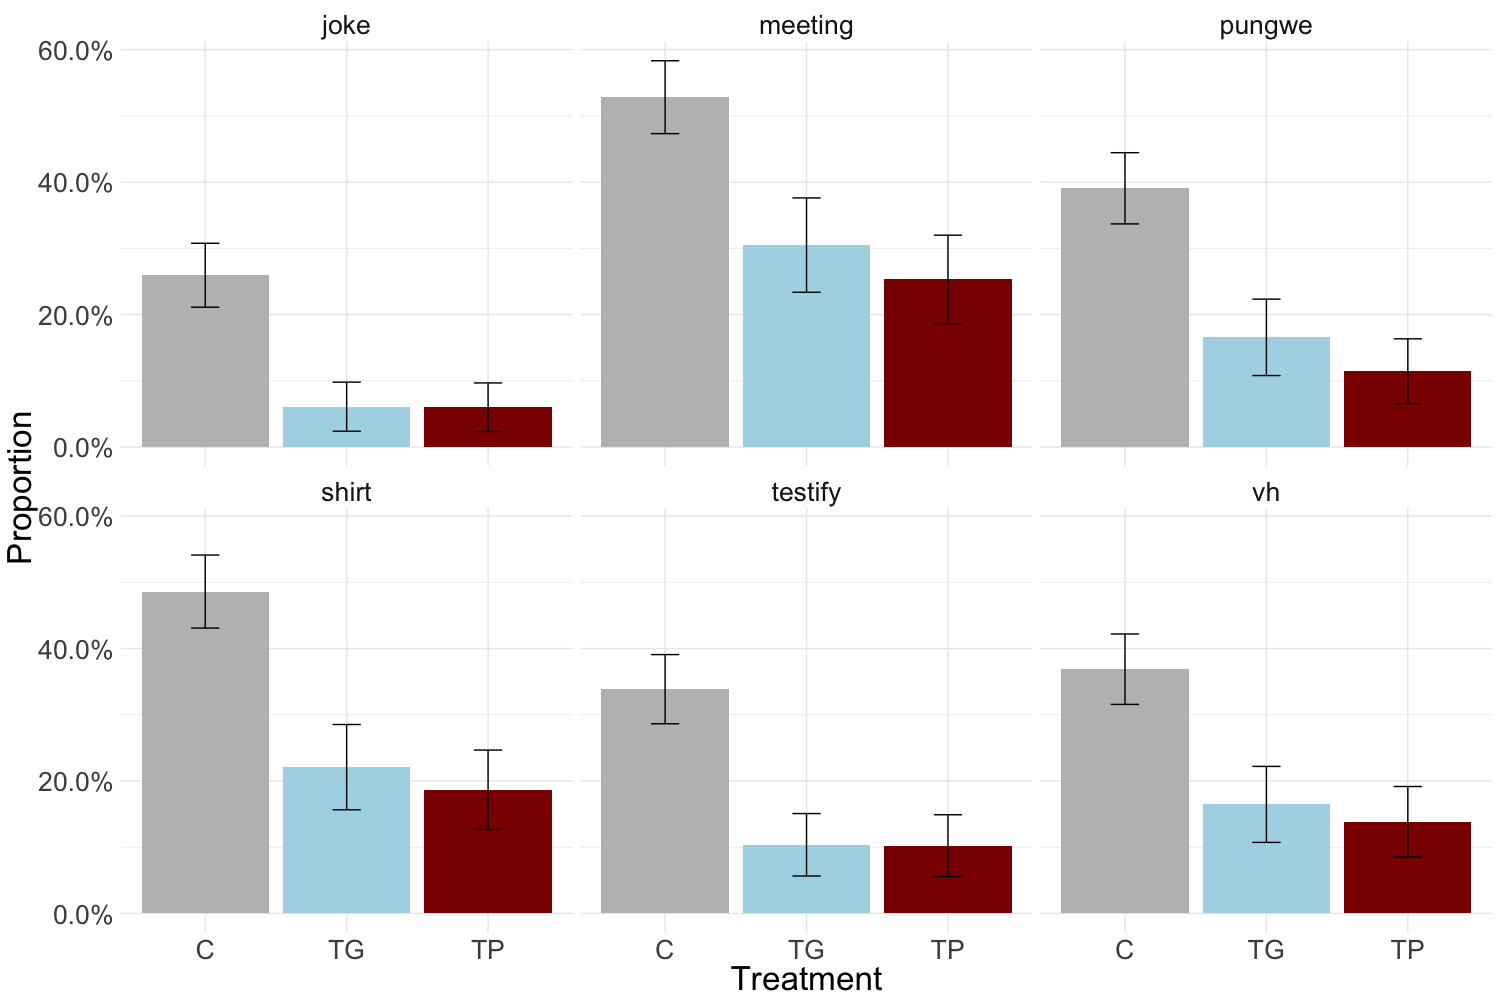
\includegraphics[scale=0.3]{Figure_2_Replicated.png}
\caption{The Fear Treatments Cause Substantively Large Increases in the Proportion of
Respondents Who Are Very Likely or Sure to Dissent During an Election Period}
\centering
\end{figure}
\newpage


\section{Mechanisms: Fear Treatments Increase Pessimism and Risk Aversion}

The author posits that fear reduces dissent through the channel of pessimism and risk aversion. In order to test the validity of these mechanisms, Young calculates the average treatment effect of the fear treatments on measures of pessimism and risk aversion. Columns 1 and 2 in Table \ref{feartreatmentmechanism} below show that the general fear treatment reduced the perceived propensity of other opposition supporters to engage in dissent by 0.32 standard deviations, while the political fear index reduced expectations of others by 0.45 standard deviations.  In real terms, while 39\% of participants in the control group believe that most or all other opposition supporters in their communities would attend an opposition rally, in the general fear treatment group just 30\% believe this and in the political fear treatment group just 20\% do.
\\


%%% Table 3

\begin{table}[!htbp] \centering 
  \caption{The Fear Treatments Increase Pessimism and Risk Aversion} 
  \label{feartreatmentmechanism} 
\scalebox{0.8}{\begin{tabular}{@{\extracolsep{5pt}}lcccccc} 
\hline \\[-1.8ex] 
\\[-1.8ex] & \multicolumn{2}{c}{Propensity of others to dissent} & \multicolumn{2}{c}{Perceived risk of repression} & \multicolumn{2}{c}{Risk aversion} \\ 
\\[-1.8ex] & General fear & Political fear & General fear & Political fear & General fear & Political fear \\ 
\\[-1.8ex] & (1) & (2) & (3) & (4) & (5) & (6)\\ 
\hline \\[-1.8ex] 
ATEs & -0.323 & -0.447 & 0.206 & 0.511 & 0.21 & 0.347 \\ 
RI p-value & 0.00059 & 0 & 0.02498 & 0 & 0.02474 & 0.00029 \\ 
N & 485 & 487 & 484 & 485 & 496 & 502 \\ 
\hline \\[-1.8ex] 
\end{tabular}}
\begin{tablenotes}
      \small
\item Notes: The first row presents the estimated Average Treatment Effects (ATEs) of the general and political fear treatments on beliefs about the likelihood that other opposition supporters will engage in dissent in Columns 1-2, on the perceived likelihood of repression in Columns 3-4, and on risk aversion in Columns 5-6. ATEs are calculated based on assignment to treatment and weighted by inverse propensity scores by block.
\end{tablenotes}
\end{table} 

\section{Replication Extension}

\subsection{Interaction of Treatment with Income}

We extend on Young's paper on the psychology of state repression by looking at the interaction between the treatment and specific characteristics of respondents in the experiment to see if the treatment had stronger or weaker effects on certain types of individuals living in electoral autocracies. The first characteristic we looked at was income which is recorded as the amount of money each earner in a household earns in a month. Table 4.0 shows that the results from this extension, whereby income is positively associated with both the hypothetical as well as the behavioral measure of dissenting behavior. However, it is not significant. Furthermore, interaction between income and treatment is not significant across any measure of dissenting behavior. This means that the fear treatment is not stronger or weaker depending on the income of respondents in the treatment group. 



\setlength{\tabcolsep}{0.3pt}
\begin{table}[!htbp] \centering 
  \caption{Effect of Treatment on Dissent by Income} 
  \label{} 
\begin{tabular}{@{\extracolsep{5pt}}lcccc} 
\\[-1.8ex]\hline 
\hline \\[-1.8ex] 
 & \multicolumn{4}{c}{\textit{Dependent variable:}} \\ 
\cline{2-5} 
\\[-1.8ex] & \multicolumn{2}{c}{Hypothetical} & \multicolumn{2}{c}{Behavioural} \\ 
\\[-1.8ex] & Political Fear & General Fear & Political Fear & General Fear\\ 
\hline \\[-1.8ex] 
 ATE & $-$0.770$^{***}$ &  & $-$0.221$^{***}$ &  \\ 
  & (0.087) &  & (0.059) &  \\ 
  & & & & \\ 
 ATE &  & $-$0.495$^{***}$ &  & $-$0.080 \\ 
  &  & (0.114) &  & (0.058) \\ 
  & & & & \\ 
 income & 0.0001  & 0.0002 & 0.0003 & 0.0003 \\ 
  & (0.0004) & (0.0004) & (0.0003) & (0.0003) \\ 
  & & & & \\ 
 Treatment*Income &  & $-$0.0004 &  & $-$0.0005 \\ 
  &  & (0.001) &  & (0.0004) \\ 
  & & & & \\ 
Treatment*Income &-0.001  &  & 0.0004 &  \\ 
  & (0.001) &  & (0.0005) &  \\ 
  & & & & \\ 
 Constant & 0.003 & $-$0.017 & 0.802$^{***}$ & 0.802$^{***}$ \\ 
  & (0.051) & (0.066) & (0.034) & (0.033) \\ 
  & & & & \\ 
\hline \\[-1.8ex] 
Observations & 486 & 483 & 325 & 328 \\ 
R$^{2}$ & 0.138 & 0.074 & 0.057 & 0.021 \\ 
Adjusted R$^{2}$ & 0.136 & 0.068 & 0.049 & 0.012 \\ 
Residual Std. Error & 1.140 (df = 484) & 1.112 (df = 479) & 0.520 (df = 321) & 0.507 (df = 324) \\ 
F Statistic & 77.584$^{***}$ (df = 1; 484) & 12.774$^{***}$ (df = 3; 479) & 6.517$^{***}$ (df = 3; 321) & 2.368$^{*}$ (df = 3; 324) \\ 
\hline 
\hline \\[-1.8ex] 
\textit{Note:}  & \multicolumn{4}{r}{$^{*}$p$<$0.1; $^{**}$p$<$0.05; $^{***}$p$<$0.01} \\ 
\end{tabular} 
\end{table} 


\subsection{Interaction of Treatment with Wealth}

In addition to the income variable, we also run the interaction with wealth of respondents in the experiment. The wealth index of each participant is constructed by adding the number of assets the household of the participant owns. Table 5.0 shows the results of this extension, whereby, the sign of wealth on the dependent variables is positive and the same as income. However, its interaction with the political fear treatment is negative and significant for the outcome of dissent in the hypothetical scenario.  


\setlength{\tabcolsep}{0.3pt}
\begin{table}[!htbp] \centering 
  \caption{Effect of Treatment on Dissent by Wealth} 
  \label{} 
\begin{tabular}{@{\extracolsep{5pt}}lcccc} 
\\[-1.8ex]\hline 
\hline \\[-1.8ex] 
 & \multicolumn{4}{c}{\textit{Dependent variable:}} \\ 
\cline{2-5} 
\\[-1.8ex] & \multicolumn{2}{c}{Hypothetical} & \multicolumn{2}{c}{Behavioural} \\ 
\\[-1.8ex] & Political Fear & General Fear & Political Fear & General Fear \\ 
\hline \\[-1.8ex] 
 ATE & $-$0.412$^{**}$ &  & $-$0.099 &  \\ 
  & (0.199) &  & (0.111) &  \\ 
  & & & & \\ 
 ATE &  & $-$0.350$^{*}$ &  & $-$0.072 \\ 
  &  & (0.209) &  & (0.116) \\ 
  & & & & \\ 
 Wealth Index & 0.026 & 0.027 & 0.015 & 0.015 \\ 
  & (0.018) & (0.017) & (0.010) & (0.010) \\ 
  & & & & \\ 
 Treatment*Wealth & $-$0.058$^{**}$ &  & $-$0.015 &  \\ 
  & (0.029) &  & (0.016) &  \\ 
  & & & & \\ 
 Treatment*Wealth &  & $-$0.029 &  & $-$0.006 \\ 
  &  & (0.032) &  & (0.018) \\ 
  & & & & \\ 
 Constant & $-$0.156 & $-$0.169 & 0.722$^{***}$ & 0.727$^{***}$ \\ 
  & (0.121) & (0.119) & (0.067) & (0.065) \\ 
  & & & & \\ 
\hline \\[-1.8ex] 
Observations & 486 & 484 & 326 & 329 \\ 
R$^{2}$ & 0.145 & 0.077 & 0.051 & 0.024 \\ 
Adjusted R$^{2}$ & 0.140 & 0.071 & 0.043 & 0.015 \\ 
Residual Std. Error & 1.137 (df = 482) & 1.110 (df = 480) & 0.524 (df = 322) & 0.508 (df = 325) \\ 
F Statistic & 27.329$^{***}$ (df = 3; 482) & 13.350$^{***}$ (df = 3; 480) & 5.818$^{***}$ (df = 3; 322) & 2.637$^{**}$ (df = 3; 325) \\ 
\hline 
\hline \\[-1.8ex] 
\textit{Note:}  & \multicolumn{4}{r}{$^{*}$p$<$0.1; $^{**}$p$<$0.05; $^{***}$p$<$0.01} \\ 
\end{tabular} 
\end{table} 

\subsection{Effect of Treatment on Pessimism and Risk Aversion by Education}

In addition to exploring the interaction of the treatment with the wealth and income of respondents in the treatment and control groups, we also extend the analysis by studying how education, age and wealth of respondents affects people's pessimism and levels of risk aversion. Table 6.0 shows that education is negatively associated with perceived likelihood of repression in both the political as well as general fear group. On the other hand, its interaction with the treatment is positively associated with pessimism and risk aversion in the general and political fear treatment respectively. This means that the treatment had a stronger effect on individuals who had higher levels of education. 

\subsection{Effect of Treatment on Pessimism and Risk Aversion by Age}

We further looked at the effect of age on the levels of pessimism and risk aversion. Table 7.0 shows that unlike education, age is positively associated with pessimism. This means that older people are likely to be more risk averse than younger participants in the experiment. However, its interaction with the treatment leads to negative association with perceived likelihood of repression as well as lower likelihood that other opposition supporters will engage in dissent. 


\subsection{Effect of Treatment on Pessimism and Risk Aversion by Wealth}

Finally, we conduct the same analysis with the wealth of participants to see if our results from Table 5.0 are robust and give the same overall results on levels of pessimism and risk aversion. As shown in Table 8.0, wealth is significantly and positively associated with perceived risk of repression, which is in line with our earlier findings in Table 5.0. Furthermore, the interaction of wealth with the treatment is significant and negative on participants' beliefs about the likelihood that other opposition supporters will engage in dissent. 


\section{Conclusion}

Our results suggest that Young's main findings of the negative effect of fear on the likelihood to dissent are robust and successfully mediated through the channels of pessimism and risk aversion in her experiment. While the characteristics of respondents studied in the extension part were not randomly assigned, we still found some interesting results. Specifically, wealth has a positive albeit insignificant association with levels of dissent. However, it becomes negative and significant when interacted with the fear treatment. Education and age, on the other hand, have opposite effects on perceived levels of repression. While higher level of education is negatively associated with the perception of repression, age is positively associated with the perceived likelihood of repression.    



\begin{landscape}
\setlength{\tabcolsep}{0.3pt}
\begin{table}[!htbp] \centering 
  \caption{Effect of Treatment on Pessimism and Risk Aversion by Education} 
  \label{} 
\begin{tabular}{@{\extracolsep{5pt}}lcccccc} 
\\[-1.8ex]\hline 
\hline \\[-1.8ex] 
 & \multicolumn{6}{c}{\textit{Dependent variable:}} \\ 
\cline{2-7} 
\\[-1.8ex] & \multicolumn{2}{c}{Propensity of Others to Dissent} & \multicolumn{2}{c}{Perceived Risk of Repression} & \multicolumn{2}{c}{Risk Aversion} \\ 
\\[-1.8ex] & Political Fear & General Fear & Political Fear & General Fear & Political Fear & General Fear\\ 
\hline \\[-1.8ex] 
 ATE & $-$0.312 &  & $-$0.165 &  & $-$0.262 &  \\ 
  & (0.258) &  & (0.252) &  & (0.253) &  \\ 
  & & & & & & \\ 
 ATE &  & $-$0.517$^{**}$ &  & $-$0.071 &  & 0.044 \\ 
  &  & (0.255) &  & (0.252) &  & (0.271) \\ 
  & & & & & & \\ 
 Education & 0.021 & 0.019 & $-$0.188$^{**}$ & $-$0.194$^{**}$ & $-$0.064 & $-$0.057 \\ 
  & (0.083) & (0.080) & (0.081) & (0.079) & (0.082) & (0.085) \\ 
  & & & & & & \\ 
 Treatment*Education & 0.002 &  & 0.203 &  & 0.280$^{**}$ &  \\ 
  & (0.142) &  & (0.138) &  & (0.139) &  \\ 
  & & & & & & \\ 
 Treatment*Education &  & 0.026 &  & 0.336$^{**}$ &  & 0.180 \\ 
  &  & (0.137) &  & (0.135) &  & (0.145) \\ 
  & & & & & & \\ 
 Constant & $-$0.034 & $-$0.032 & 0.320$^{**}$ & 0.335$^{**}$ & $-$0.032 & $-$0.046 \\ 
  & (0.154) & (0.150) & (0.150) & (0.148) & (0.152) & (0.159) \\ 
  & & & & & & \\ 
\hline \\[-1.8ex] 
Observations & 485 & 487 & 484 & 485 & 496 & 502 \\ 
R$^{2}$ & 0.022 & 0.054 & 0.020 & 0.079 & 0.019 & 0.031 \\ 
Adjusted R$^{2}$ & 0.016 & 0.048 & 0.013 & 0.073 & 0.013 & 0.025 \\ 
Residual Std. Error & 1.208 (df = 481) & 1.180 (df = 483) & 1.180 (df = 480) & 1.162 (df = 481) & 1.206 (df = 492) & 1.255 (df = 498) \\ 
F Statistic & 3.675$^{**}$ (df = 3; 481) & 9.154$^{***}$ (df = 3; 483) & 3.198$^{**}$ (df = 3; 480) & 13.702$^{***}$ (df = 3; 481) & 3.114$^{**}$ (df = 3; 492) & 5.335$^{***}$ (df = 3; 498) \\ 
\hline 
\hline \\[-1.8ex] 
\textit{Note:}  & \multicolumn{6}{r}{$^{*}$p$<$0.1; $^{**}$p$<$0.05; $^{***}$p$<$0.01} \\ 
\end{tabular} 
\end{table} 
\end{landscape}

\begin{landscape}
\setlength{\tabcolsep}{0.3pt}
\begin{table}[!htbp] \centering 
  \caption{Effect of Treatment on Pessimism and Risk Aversion by Age} 
  \label{} 
\begin{tabular}{@{\extracolsep{5pt}}lcccccc} 
\\[-1.8ex]\hline 
\hline \\[-1.8ex] 
 & \multicolumn{6}{c}{\textit{Dependent variable:}} \\ 
\cline{2-7} 
\\[-1.8ex] & \multicolumn{2}{c}{Propensity of Others to Dissent} & \multicolumn{2}{c}{Perceived Risk of Repression} & \multicolumn{2}{c}{Risk Aversion} \\ 
\\[-1.8ex] & Political Fear & General Fear & Political Fear & General Fear & Political Fear & General Fear\\ 
\hline \\[-1.8ex] 
 ATE & $-$0.153 &  & 0.794$^{***}$ &  & 0.330 &  \\ 
  & (0.277) &  & (0.273) &  & (0.275) &  \\ 
  & & & & & & \\ 
 ATE &  & $-$0.024 &  & 0.515$^{*}$ &  & 0.495$^{*}$ \\ 
  &  & (0.271) &  & (0.267) &  & (0.285) \\ 
  & & & & & & \\ 
 Age & 0.006 & 0.006 & 0.009$^{**}$ & 0.010$^{**}$ & $-$0.005 & $-$0.005 \\ 
  & (0.004) & (0.004) & (0.004) & (0.004) & (0.004) & (0.004) \\ 
  & & & & & & \\ 
 Treatment*Age & $-$0.004 &  & $-$0.016$^{**}$ &  & $-$0.003 &  \\ 
  & (0.007) &  & (0.007) &  & (0.007) &  \\ 
  & & & & & & \\ 
 Treatment*Age &  & $-$0.012$^{*}$ &  & $-$0.0001 &  & $-$0.003 \\ 
  &  & (0.007) &  & (0.007) &  & (0.007) \\ 
  & & & & & & \\ 
 Constant & $-$0.243 & $-$0.238 & $-$0.365$^{**}$ & $-$0.369$^{**}$ & 0.035 & 0.039 \\ 
  & (0.163) & (0.158) & (0.159) & (0.155) & (0.162) & (0.167) \\ 
  & & & & & & \\ 
\hline \\[-1.8ex] 
Observations & 485 & 487 & 484 & 485 & 496 & 502 \\ 
R$^{2}$ & 0.028 & 0.060 & 0.023 & 0.082 & 0.017 & 0.035 \\ 
Adjusted R$^{2}$ & 0.022 & 0.055 & 0.017 & 0.076 & 0.011 & 0.029 \\ 
Residual Std. Error & 1.205 (df = 481) & 1.176 (df = 483) & 1.178 (df = 480) & 1.160 (df = 481) & 1.207 (df = 492) & 1.253 (df = 498) \\ 
F Statistic & 4.570$^{***}$ (df = 3; 481) & 10.347$^{***}$ (df = 3; 483) & 3.750$^{**}$ (df = 3; 480) & 14.309$^{***}$ (df = 3; 481) & 2.823$^{**}$ (df = 3; 492) & 6.022$^{***}$ (df = 3; 498) \\ 
\hline 
\hline \\[-1.8ex] 
\textit{Note:}  & \multicolumn{6}{r}{$^{*}$p$<$0.1; $^{**}$p$<$0.05; $^{***}$p$<$0.01} \\ 
\end{tabular} 
\end{table}
\end{landscape}


\begin{landscape}
\setlength{\tabcolsep}{0.3pt}
\begin{table}[!htbp] \centering 
  \caption{Effect of Treatment on Pessimism and Risk Aversion by Wealth} 
  \label{} 
\begin{tabular}{@{\extracolsep{5pt}}lcccccc} 
\\[-1.8ex]\hline 
\hline \\[-1.8ex] 
 & \multicolumn{6}{c}{\textit{Dependent variable:}} \\ 
\cline{2-7} 
\\[-1.8ex] & \multicolumn{2}{c}{Propensity of Others to Dissent} & \multicolumn{2}{c}{Perceived Risk of Repression} & \multicolumn{2}{c}{Risk Aversion} \\ 
\\[-1.8ex] & Political Fear & General Fear & Political Fear & General Fear & Political Fear & General Fear \\
\hline \\[-1.8ex] 
 ATE & 0.037 &  & 0.206 &  & 0.233 &  \\ 
  & (0.227) &  & (0.220) &  & (0.224) &  \\ 
  & & & & & & \\ 
 ATE &  & 0.003 &  & 0.436$^{**}$ &  & 0.056 \\ 
  &  & (0.206) &  & (0.202) &  & (0.216) \\ 
  & & & & & & \\ 
 Wealth Index & 0.026 & 0.024 & 0.060$^{***}$ & 0.060$^{***}$ & $-$0.023 & $-$0.022 \\ 
  & (0.019) & (0.018) & (0.018) & (0.018) & (0.019) & (0.019) \\ 
  & & & & & & \\ 
 Treatment*Wealth Index & $-$0.057$^{*}$ &  & $-$0.001 &  & $-$0.005 &  \\ 
  & (0.034) &  & (0.033) &  & (0.034) &  \\ 
  & & & & & & \\ 
 Treatment*Wealth Index &  & $-$0.077$^{**}$ &  & 0.015 &  & 0.049 \\ 
  &  & (0.030) &  & (0.030) &  & (0.031) \\ 
  & & & & & & \\ 
 Constant & $-$0.161 & $-$0.148 & $-$0.379$^{***}$ & $-$0.380$^{***}$ & $-$0.001 & $-$0.011 \\ 
  & (0.129) & (0.125) & (0.125) & (0.122) & (0.128) & (0.131) \\ 
  & & & & & & \\ 
\hline \\[-1.8ex] 
Observations & 485 & 487 & 484 & 485 & 496 & 502 \\ 
R$^{2}$ & 0.028 & 0.066 & 0.039 & 0.104 & 0.015 & 0.033 \\ 
Adjusted R$^{2}$ & 0.022 & 0.060 & 0.033 & 0.099 & 0.009 & 0.027 \\ 
Residual Std. Error & 1.205 (df = 481) & 1.172 (df = 483) & 1.169 (df = 480) & 1.146 (df = 481) & 1.208 (df = 492) & 1.254 (df = 498) \\ 
F Statistic & 4.698$^{***}$ (df = 3; 481) & 11.428$^{***}$ (df = 3; 483) & 6.470$^{***}$ (df = 3; 480) & 18.647$^{***}$ (df = 3; 481) & 2.517$^{*}$ (df = 3; 492) & 5.657$^{***}$ (df = 3; 498) \\ 
\hline 
\hline \\[-1.8ex] 
\textit{Note:}  & \multicolumn{6}{r}{$^{*}$p$<$0.1; $^{**}$p$<$0.05; $^{***}$p$<$0.01} \\ 
\end{tabular} 
\end{table} 
\end{landscape}

\newpage
\bibliography{reference}

\end{document}